%!TEX root = ../ArticleCalib_main.tex


%%%%%%%%%%%%% STATS MEAN COL AND LINE CIC AND IDARK

\begin{figure}[htbp]
\begin{center}
\captionsetup[subfigure]{position=top, labelfont=bf, textfont=normalfont, singlelinecheck=off, justification=raggedright }

\subfloat[]{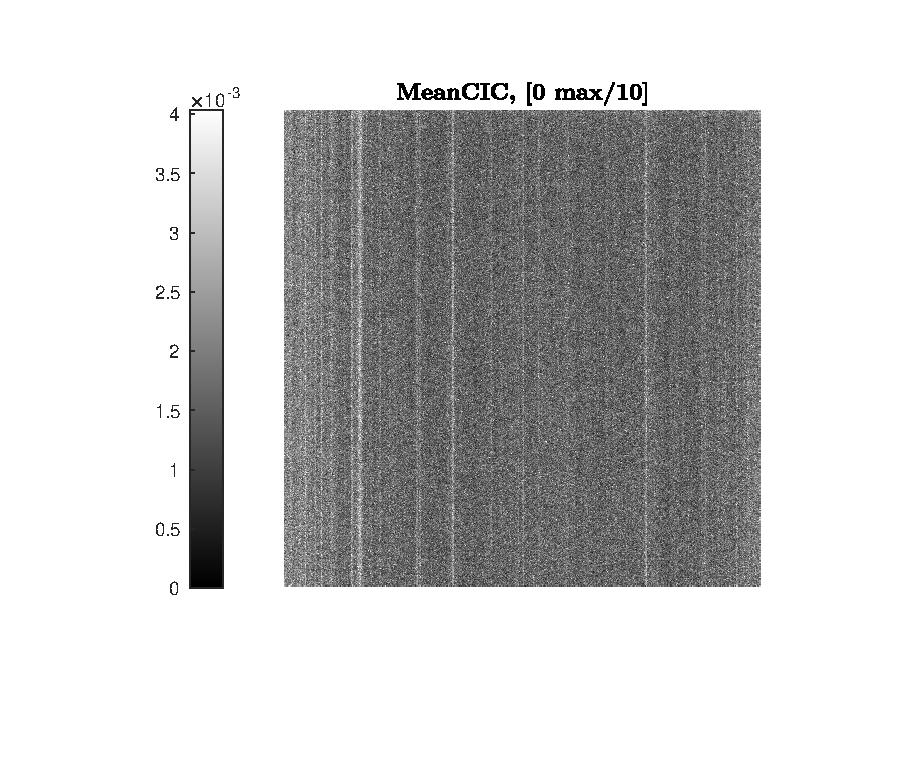
\includegraphics[width=0.49\linewidth]{fig1sup_caract_LinesColResponse/fig11Asup_ImCICmax10.eps}\label{fig:LinesColCIC:A}} \qquad
\subfloat[]{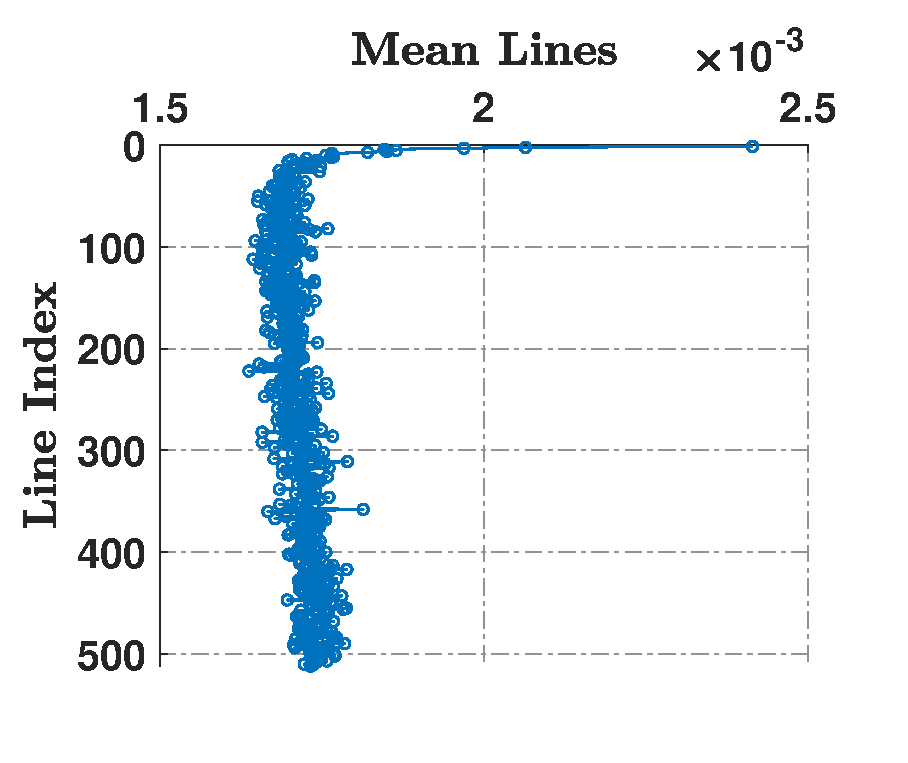
\includegraphics[width=0.4\linewidth]{fig1sup_caract_LinesColResponse/fig11Bsup_ColMean_LineMatCIC_invaxes.eps}\label{fig:LinesColCIC:B}} \\

\subfloat[]{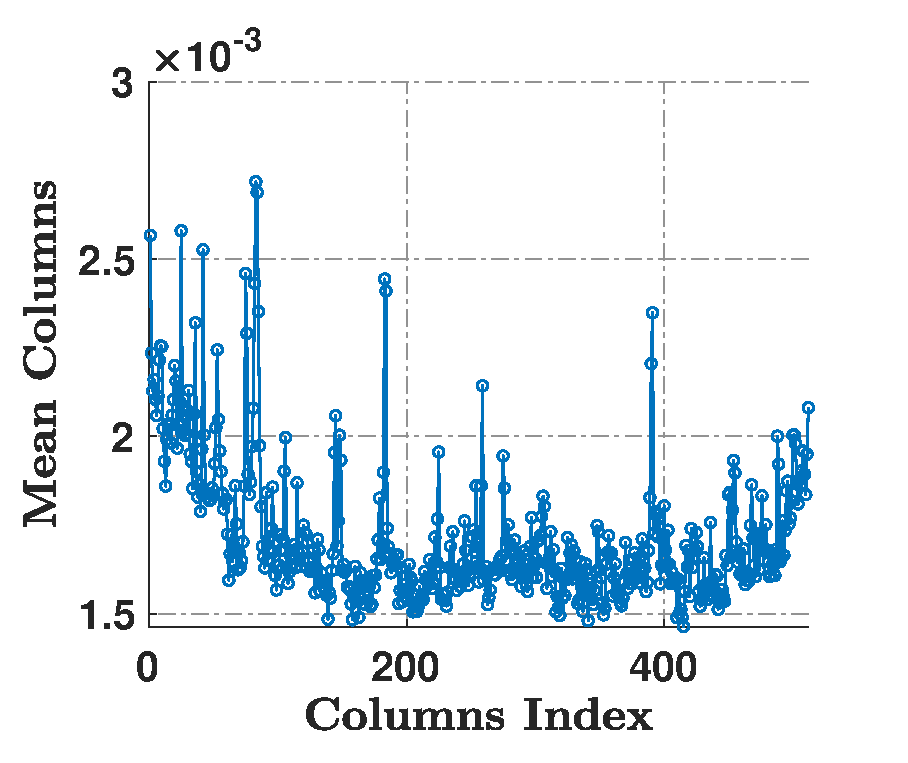
\includegraphics[width=0.4\linewidth]{fig1sup_caract_LinesColResponse/fig11Csup_RowMean_ColumnMatCIC.eps}\label{fig:LinesColCIC:C}} \qquad \qquad \qquad \qquad \qquad \qquad \qquad \qquad \qquad \qquad  



\caption{{\bf Lines and Column Pattern for CIC}.  
 Image of the CIC mean with a maximum threshold set to $1/10^e$ of the maximal pixel value.(\subref{fig:LinesColCIC:A}.)
Profile of the CIC lines (mean) (\subref{fig:LinesColCIC:B}.)
Profile of the CIC columns (mean)(\subref{fig:LinesColCIC:C}.)}
\label{fig:BBRtheo1}
\end{center}
\end{figure}


\begin{figure}[htbp]
\begin{center}
\captionsetup[subfigure]{position=top, labelfont=bf, textfont=normalfont, singlelinecheck=off, justification=raggedright }

\subfloat[]{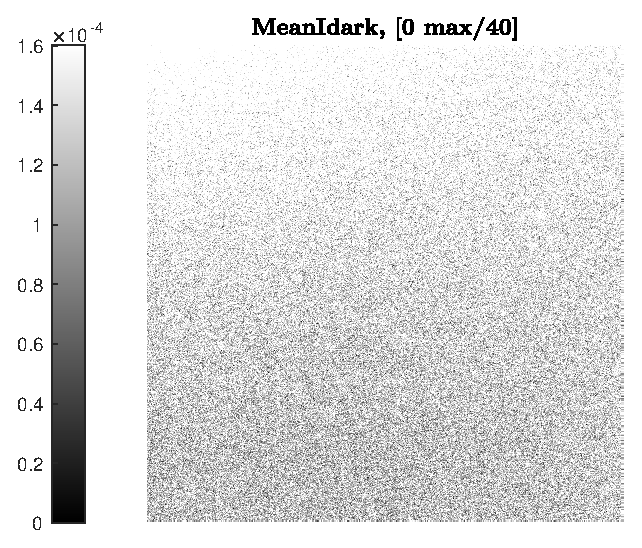
\includegraphics[width=0.35\linewidth]{fig1sup_caract_LinesColResponse/fig12Bsup_ImIdmax40.eps}\label{fig:LinesColId:A}} \qquad
\subfloat[]{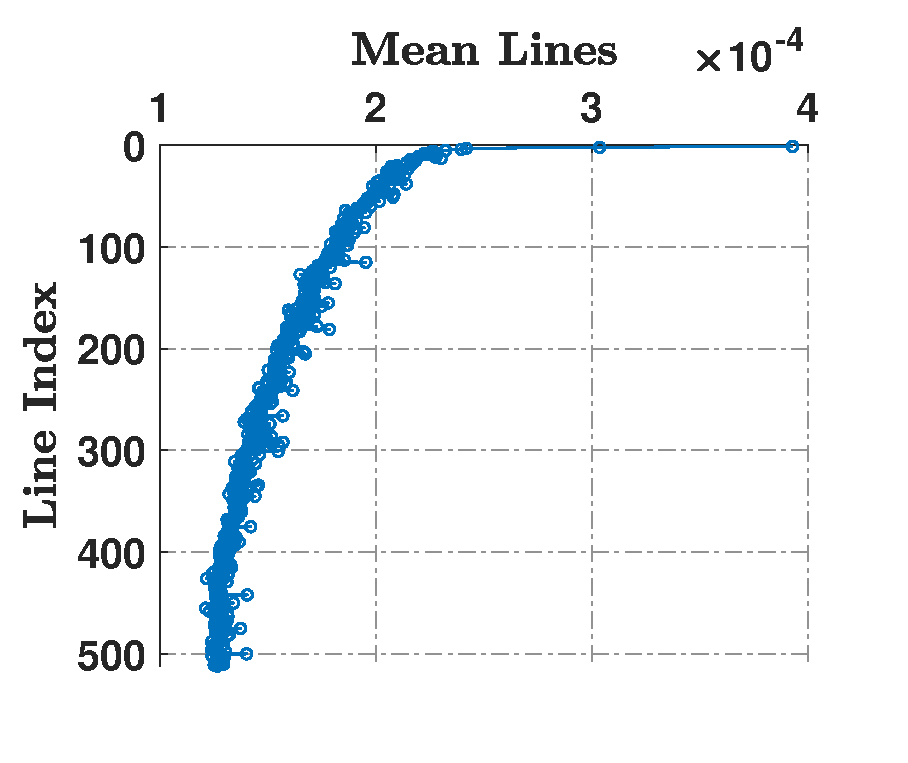
\includegraphics[width=0.4\linewidth]{fig1sup_caract_LinesColResponse/fig12Bsup_ColMean_LineMatId_invaxes.eps}\label{fig:LinesColId:B}} \\


\subfloat[]{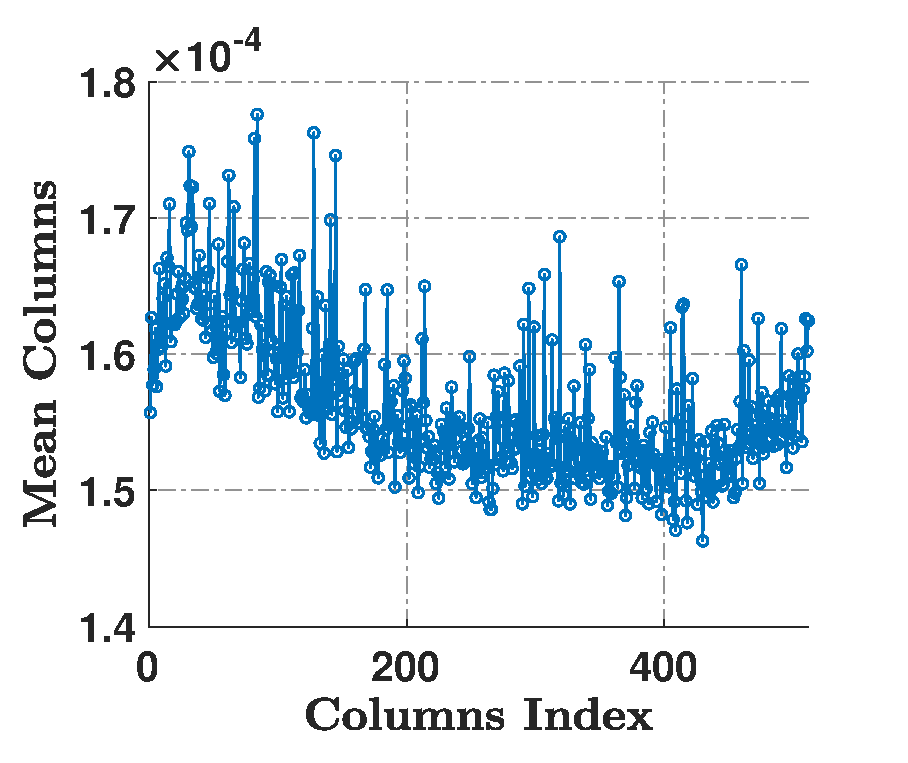
\includegraphics[width=0.4\linewidth]{fig1sup_caract_LinesColResponse/fig12Csup_RowMean_ColumnMatId.eps}\label{fig:LinesColId:C}} \qquad
\subfloat[]{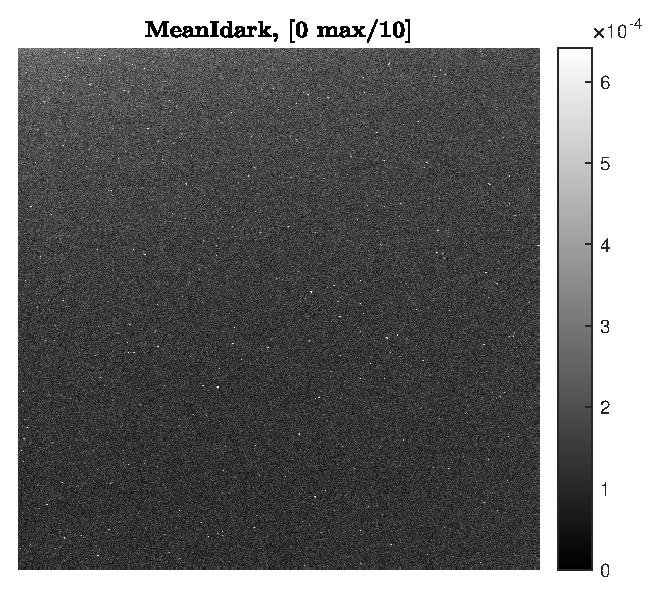
\includegraphics[width=0.35\linewidth]{fig1sup_caract_LinesColResponse/fig12Asup_ImIdmax10.eps}\label{fig:LinesColId:D}} 



\caption{{\bf Lines and Column Pattern for Id}.  
  Image of the Id mean with a maximum threshold set to $1/40^e$ of the maximal pixel value.(\subref{fig:LinesColId:A}.)
  Profile of the Id lines (mean) (\subref{fig:LinesColId:B}.)
  Profile of the Id columns (mean) (\subref{fig:LinesColId:C}.)
  Image of the Id mean with a maximum threshold set to $1/10^e$ of the maximal pixel value.(\subref{fig:LinesColId:D}.)}
\label{fig:BBRtheo1}
\end{center}
\end{figure}

